% !TEX root = ./article.tex

\documentclass{article}

\usepackage{mystyle}
\usepackage{myvars}



%-----------------------------

\begin{document}

	\maketitle % Insert title

	\thispagestyle{fancy} % All pages have headers and footers


%-----------------------------
%	ABSTRACT
%-----------------------------

	\begin{abstract}
		\noindent [TODO ]
	\end{abstract}

%-----------------------------
%	TEXT
%-----------------------------


	\section{Introducción}
	\label{sec:introducción}

		\paragraph{}
		[TODO]

		\subsection{Regresión Lineal Múltiple}

			\paragraph{}
			[TODO]



		\subsection{Regresión Logística}

			\paragraph{}
			[TODO]




	\section{Evaluación de resultados a partir de distintas cotas de error relativo para Regresión Lineal Múltiple}
	\label{sec:e1}

		\paragraph{}
		En esta sección se realiza un experimento para estudiar la evolución de la tasa de error conforme aumenta la cota de error relativo fijada para admitir una instancia como clasificada de manera correcta. El algoritmo utilizado es el de Regresión Lineal Múltiple mediante el aprendizaje por mínimos cuadrados descrito anteriormente.

		\paragraph{}
		El conjunto de datos que se ha utilizado para dichos experimentos es \textbf{Housing Data Set} \cite{dataset:housing}, que está formado por \textbf{506 instancias}. Dichas instancias contienen \textbf{13 atributos} de carácter númerico. La \textbf{clase de destino es de carácter numérico} (por lo que es una regresión y no una clasificación). En cuanto a la metodología experimental, se ha seguido una extrategia de \textbf{HoldOut} con particionamiento de los datos de manera que $\frac{2}{3}$ son utilizados en la fase de entrenamiento y $\frac{1}{3}$ en la de test.

		\paragraph{}
		Los resultados obtenidos tras los experimentos se muestran de manera tabular en la tabla \ref{table:e1} mientras que se puede apreciar la evolución conforme aumenta el rango de la cota de error de manera gráfica en la figura \ref{plot:e1}.

		\begin{figure}[h]
			\begin{center}
				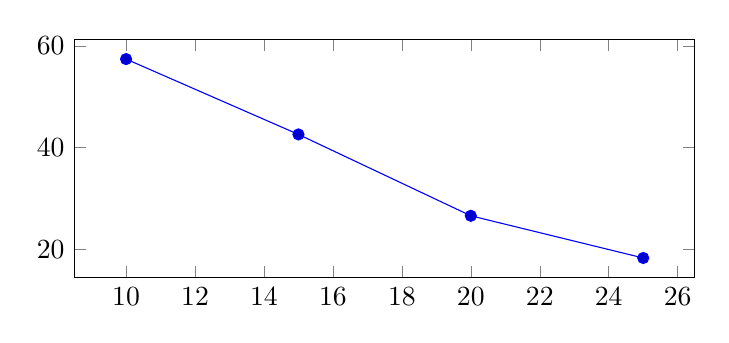
\begin{tikzpicture}
					\begin{axis}[
						% only scale the axis, not the axis including the ticks and labels
						scale only axis=true,
						% set `width' and `height' to the desired values
						width=0.65\textwidth,
						height=0.25\textwidth,
						]
						\addplot coordinates {
							(10,57.396)
							(15,42.604)
							(20,26.627)
							(25,18.343)
						};
					\end{axis}
				\end{tikzpicture}
			\end{center}
			\caption{Evolución de la tasa de error para la \emph{Regresión Lineal Múltiple} sobre el conjunto de datos \emph{Housing} conforme aumenta la cota máxima de error relativo}
			\label{plot:e1}
		\end{figure}

		\begin{table}[h]
			\centering
			\small
			\begin{tabu}{ | c | c | c | c | c | }
				\hline
					& \multicolumn{4}{ c | }{Regresión --- Housing Dataset} \\ \hline
					& \emph{Lineal 10\%} & \emph{Lineal 15\%} & \emph{Lineal 20\%} & \emph{Lineal 25\%}\\ \cline{2-5}
				Error HoldOut						& $57.396\%$	 & $42.604\%$ & $26.627\%$ & $18.343\%$ \\
				\hline
			\end{tabu}
			\caption{Evolución de la tasa de error para la \emph{Regresión Lineal Múltiple} sobre el conjunto de datos \emph{Housing} conforme aumenta la cota máxima de error relativo}
			\label{table:e1}
		\end{table}

	\section{Comparación de resultados entre Regresión Logística y Regresión Lineal Múltiple}
	\label{sec:e2}

		\paragraph{}
		En esta sección se realiza un experimento para estudiar la tasa de error obtenida mediante la estrategia de \emph{Regresión Logística} para después compararla con los resultados obtenidos mediante la estrategia de \emph{Regresión Lineal}. Dicha labor es posible cuando la clase de destino es numérica pero se puede discretizar. (En este caso es de carácter entero y acotada por lo que su discretización es trivial). Puesto que no es de tipo binario es necesario seguir la estrategía de clasificación por pares tal y como se ha descrito anteriormente.

		\paragraph{}
		El conjunto de datos que se ha utilizado para dichos experimentos es \textbf{Wine Data Set} \cite{dataset:wine}, formado por \textbf{178 instancias}. Dichas instancias contienen \textbf{12 atributos} de carácter númerico. La \textbf{clase de destino es de carácter numérico}. Sin embargo, en este caso es de tipo entero, por lo que puede ser vista como una variable categórica. En cuanto a la metodología experimental, se ha seguido una extrategia de \textbf{HoldOut} con particionamiento de los datos de manera que $\frac{2}{3}$ son utilizados en la fase de entrenamiento y $\frac{1}{3}$ en la de test.

		\paragraph{}
		Los resultados obtenidos tras los experimentos se muestran de manera tabular en la tabla \ref{table:e2}. Además, se muestran de manera gráfica en la figura \ref{plot:e2}.


		\begin{figure}[h]
			\begin{center}
				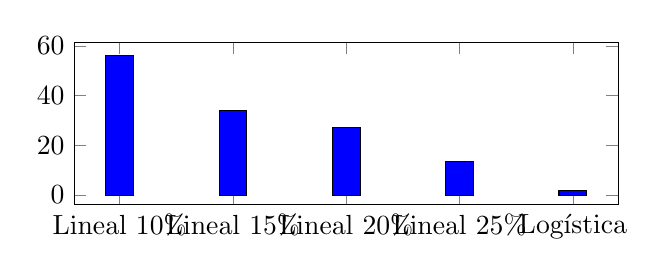
\begin{tikzpicture}
					\begin{axis}[
						symbolic x coords={Lineal 10\%,Lineal 15\%,Lineal 20\%,Lineal 25\%,Logística},
						width=0.7\textwidth,
						height=0.3\textwidth,
						xtick=data]
						\addplot[ybar, fill=blue] coordinates {
							(Lineal 10\%, 55.932)
							(Lineal 15\%, 33.898)
							(Lineal 20\%, 27.119)
							(Lineal 25\%, 13.559)
							(Logística, 1.6949)
						};
					\end{axis}
				\end{tikzpicture}
			\end{center}
			\caption{Resultados obtenidos a nivel de tasa de error mediante \emph{Regresión Lineal Múltiple} y \emph{Regresión Logística} sobre el conjunto de datos \emph{Wine}}
			\label{plot:e2}
		\end{figure}

		\begin{table}[h]
			\centering
			\small
			\begin{tabu}{ | c | c | c | c | c | c | }
				\hline
					& \multicolumn{5}{ c | }{Regresión --- Wine Dataset} \\ \hline
					&\emph{Lineal 10\%} & \emph{Lineal 15\%} & \emph{Lineal 20\%} & \emph{Lineal 25\%} & \emph{Logística}\\ \cline{2-6}
				Error HoldOut	& $55.932\%$	 & $33.898\%$ & $27.119\%$ & $13.559\%$	& $1.6949\%$ \\
				\hline
			\end{tabu}
			\caption{Resultados obtenidos a nivel de tasa de error mediante \emph{Regresión Lineal Múltiple} y \emph{Regresión Logística} sobre el conjunto de datos \emph{Wine}}
			\label{table:e2}
		\end{table}

		\paragraph{}
		Tal y como se puede apreciar tras analizar los resultados, a través de la \emph{Regresión Logística} se obtienen resultados mucho más óptimos. Sin embargo, para aplicar dicha técnica es necesario que la clase de destino esté discretizada. Además conlleva un mayor coste computacional derivado de la estrategia de clasificación por pares, que incrementa en un orden cuadrático los costes conforme aumentan el número de clases de destino.



%-----------------------------
%	Bibliographic references
%-----------------------------
	\nocite{garciparedes:machine-learning-regression}
	\nocite{subject:taa}
	\nocite{tool:weka}
  \bibliographystyle{alpha}
  \bibliography{bib/misc}

\end{document}
